\section{Test}
\subsection{CLI}
\begin{enumerate}
  \item \textbf{Esecuzione del client con server offline} \\ \\
  \begin{minipage}[t]{0.3\textwidth}
    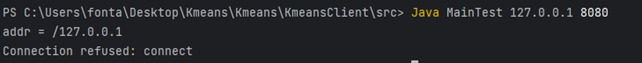
\includegraphics[scale=0.8]{img/test1.png}
  \end{minipage}
  \item \textbf{Esecuzione senza parametri}: il programma deve essere avviato fornendo come parametri l'indirizzo IP/DNS del server e la porta logica. Se si lavora con la stessa macchina si può inserire come primo parametro localhost, 127.0.0.1 (indirizzo IPv4 locale) oppure ::1 (indirizzo IPv6 locale). \\ \\
  \begin{minipage}[t]{0.3\textwidth}
    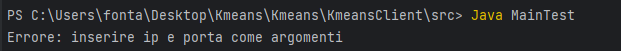
\includegraphics[scale=0.8]{img/test2.png}
  \end{minipage}
  \item \textbf{Esecuzione con porta errata}: la porta logica è un numero a 16 bit, dunque un decimale compreso tra 0 e 65.535. \\ \\
  \begin{minipage}[t]{0.3\textwidth}
    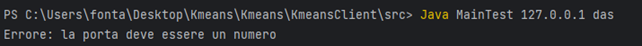
\includegraphics[scale=0.8]{img/test3.png}
  \end{minipage}
  \item \textbf{Esecuzione con IP/DNS inesistente}: in questa esecuzione il server non esiste e dunque il client non riesce a connettersi. In particolare il programma si connette a un server DNS per convertire l'indirizzo fornito in un indirizzo IP ma tale indirizzo non è registrato e dunque si ha errore. \\ \\
  \begin{minipage}[t]{0.3\textwidth}
    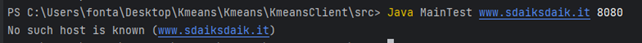
\includegraphics[scale=0.8]{img/test4.png}
  \end{minipage}
  \item \textbf{Esecuzione con parametri corretti}: quando il programma viene eseguito nelle condizioni funzionali (quindi server avviato e parametri validi) vengono stampati a schermo indirizzo IP e porta del server, seguiti dalla porta che sta usando il processo per la comunicazione. Viene poi mostrato all'utente un menù con due opzioni. L'opzione (1) permetterà al client di caricare un cluster di dati che è stato serializzato sul server come un file, mentre l'opzione (2) consente di creare un nuovo cluster di dati mediante l'algoritmo del K-means. In caso di input non validi viene chiesto all'utente di reinserire finchè non si avrà un'opzione valida.  \\ \\
  \begin{minipage}[t]{0.3\textwidth}
    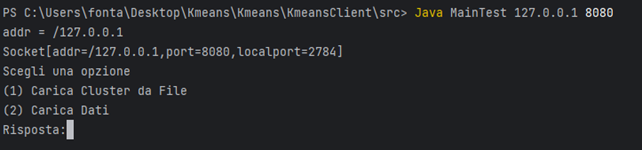
\includegraphics[scale=0.8]{img/test5.png}
  \end{minipage}
  \\
  \begin{minipage}[t]{0.3\textwidth}
    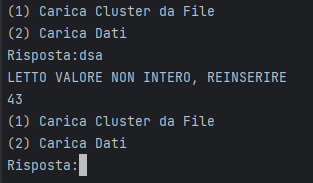
\includegraphics[scale=0.8]{img/test6.png}
  \end{minipage}
  \begin{itemize}[label=-]
    \item \textbf{Opzione (1)}: Viene chiesto all'utente di inserire il nome del database, della tabella e del numero di cluster creati. Il server andrà dunque a cercare il file corrispondente a tali informazioni e, se non trovato, manderà un messaggio di errore all'utente (come nell'esempio). Viene chiesto all'utente se vuole tornare al menù oppure terminare l'esecuzione del programma. Se viene digitato \textit{n} il programma termina. Nel caso in cui il file corrispondente alle richieste esista viene inviato al client il contenuto del file, ovvero i centroidi dei cluster. \\ \\
    \begin{minipage}[t]{0.3\textwidth}
      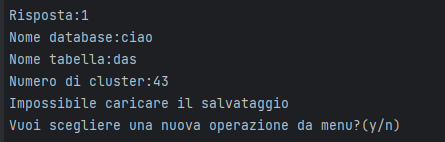
\includegraphics[scale=0.8]{img/test7.png}
    \end{minipage}
    \\
    \begin{minipage}[t]{0.3\textwidth}
      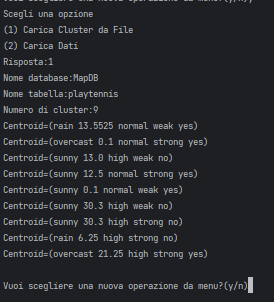
\includegraphics[scale=0.8]{img/test8.png}
    \end{minipage}
    \item \textbf{Opzione (2)}: Viene chiesto all'utente se vuole usare i valori di default o meno:
    \begin{itemize}[label=-]
      \item \textbf{Valori di default}: i valori di default sono:
      \begin{itemize}[label=-]
        \item localhost $\rightarrow$ server database
        \item 3306 $\rightarrow$ porta dabasase
        \item MapDB $\rightarrow$ nome database
        \item playtennis $\rightarrow$ nome tabella
        \item MapUser $\rightarrow$ nome utente
        \item password di MapUser
      \end{itemize}
      \begin{minipage}[t]{0.3\textwidth}
        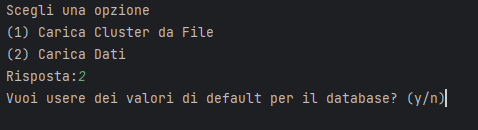
\includegraphics[scale=0.8]{img/test9.png}
      \end{minipage}
      \\ Nel caso di risposta affermativa viene chiesto all'utente il numero dei cluster. Una volta confermati (se questi sono validi) il server eseguirà l'algoritmo di K-means e invierà il risultato al client. Viene poi chiesto se si vuole riprendere l'esecuzione sullo stesso dataset o meno. \\ \\
      \begin{minipage}[t]{0.3\textwidth}
        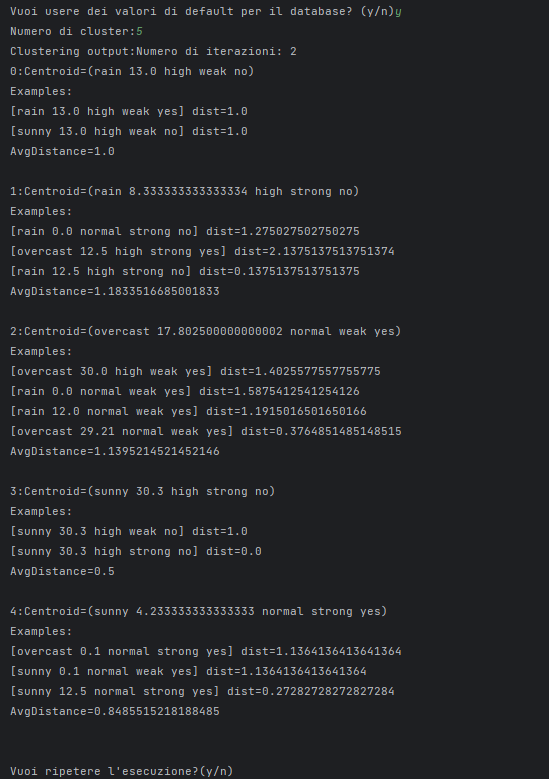
\includegraphics[scale=0.8]{img/test10.png}
      \end{minipage}
      \\ Se l'utente non vuole ripetere l'esecuzione sul dataset ha due scelte:
      \begin{enumerate}
        \item Tornare al menù
        \item Terminare l'esecuzione
      \end{enumerate}
      \begin{minipage}[t]{0.3\textwidth}
        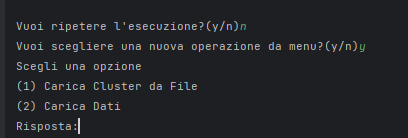
\includegraphics[scale=0.8]{img/test12.png}
      \end{minipage}
      \item \textbf{Valori non di default}: l'utente può scegliere di non usare i valori di default. In quel caso deve inserire tutte le informazioni necessarie. In caso di valori non validi verrà segnalato l'errore all'utente, il quale sceglierà se proseguire con i valori di default oppure se riprovare a inserire dei valori personalizzati. L'uso di valori personalizzati permette di utilizzare dataset già presenti nel server del database. \\ \\
      \begin{minipage}[t]{0.3\textwidth}
        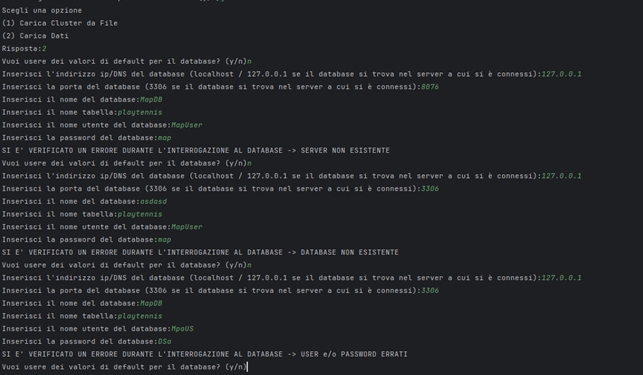
\includegraphics[scale=0.8]{img/test13.png}
      \end{minipage}
    \end{itemize} 
    Ogni volta che l'utente richiede la creazione di un dataset al server, quest'ultimo serializzerà i cluster in un file con nome del tipo: \textbf{\textit{NomedatabaseNometabellaNumerocluster.dat}}. \\ \\
    \begin{minipage}[t]{0.3\textwidth}
      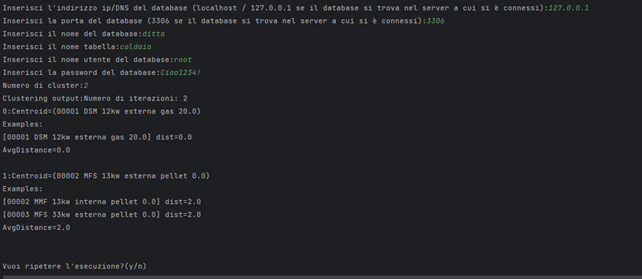
\includegraphics[scale=0.8]{img/test14.png}
    \end{minipage}
  \end{itemize}
\end{enumerate}

\subsection{App}
\begin{enumerate}
  \item \textbf{Esecuzione del client senza inserire tutti i parametri}: nel caso in cui nella schermata di apertura l'utente non inserisca tutti i parametri richiesti, riceverà un messaggio di errore.
  \begin{figure}[H]
    \centering
    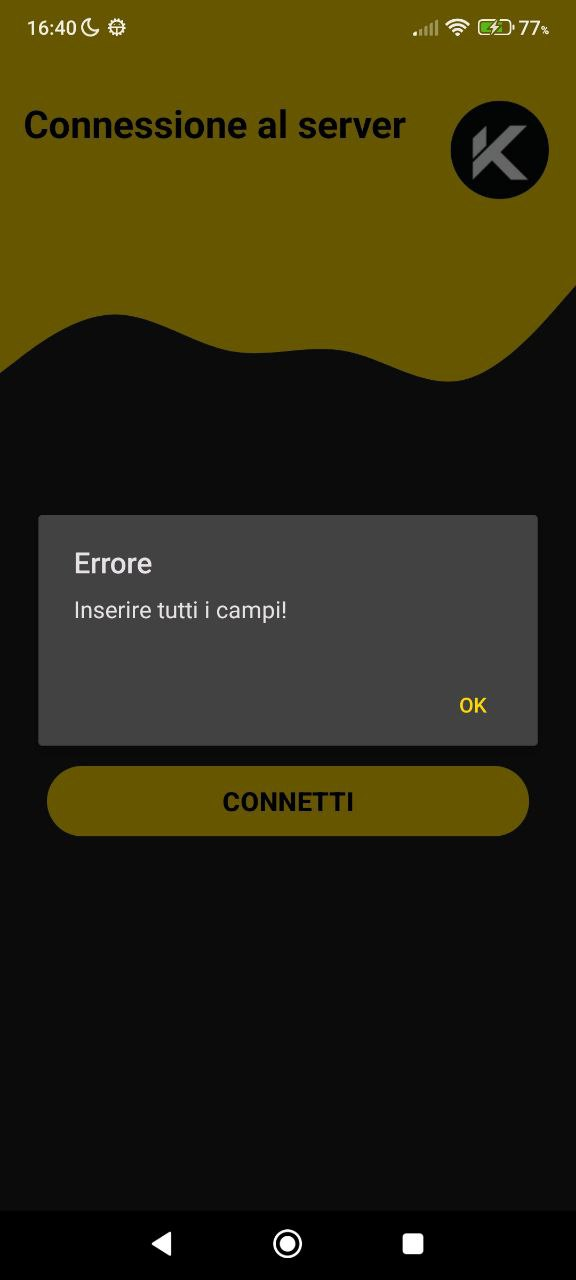
\includegraphics[scale=0.2]{img/app3.png}
  \end{figure}
  \item \textbf{Esecuzione del client con server offline, con porta errata, con IP/DNS inesistente o con telefono offline}: una volta inseriti i dati, verranno richiesti all'utente le informazioni riguardanti il database. A questo punto l'utente proverà a connettersi al server e al database, ricevendo un messaggio di errore:
  \begin{figure}[H]
    \centering
    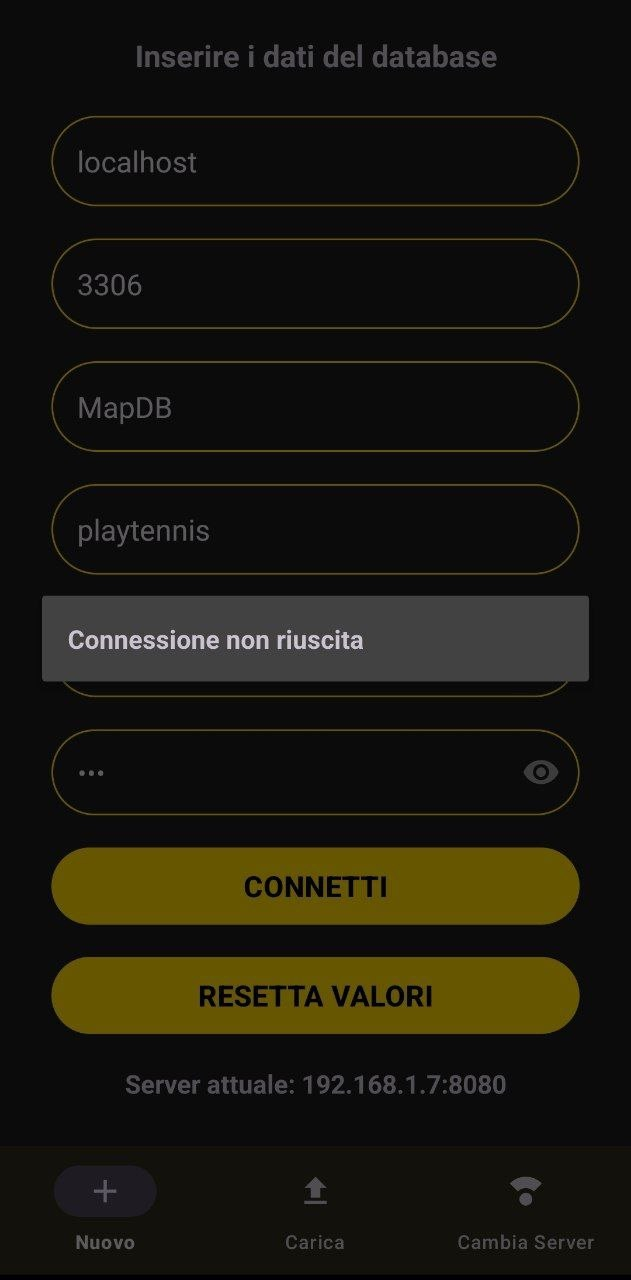
\includegraphics[scale=0.2]{img/app2.png}
  \end{figure}
  \item \textbf{Esecuzione con parametri corretti}: quando il server è avviato e vengono immessi i parametri corretti all'avvio dell'applicazione (o tramite l'apposito tab per cambiare server) l'utente può connettersi al database. 
  \begin{itemize}[label=-]
    \item \textbf{Connessione al database}: se l'utente inserisce i parametri del database corretti l'applicazione si connetterà al server e darà la possibilità all'utente di selezionare il numero di cluster.
    \begin{figure}[H]
      \centering
      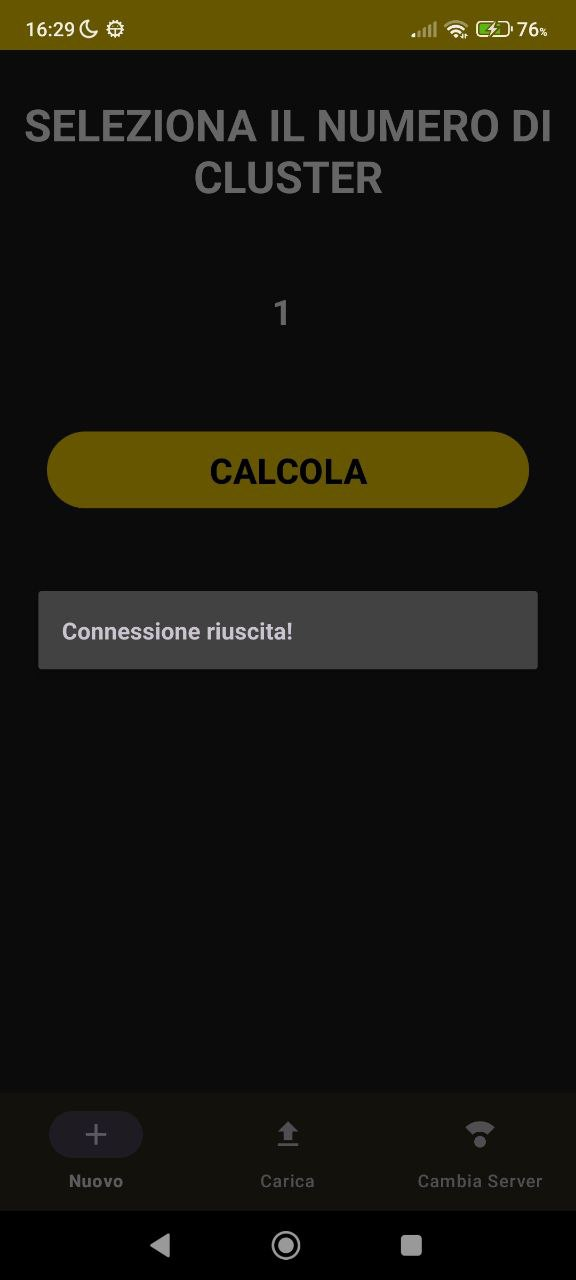
\includegraphics[scale=0.2]{img/app4.png}
    \end{figure}
    Se l'utente non compila tutti i campi, riceverà un errore.
    \begin{figure}[H]
      \centering
      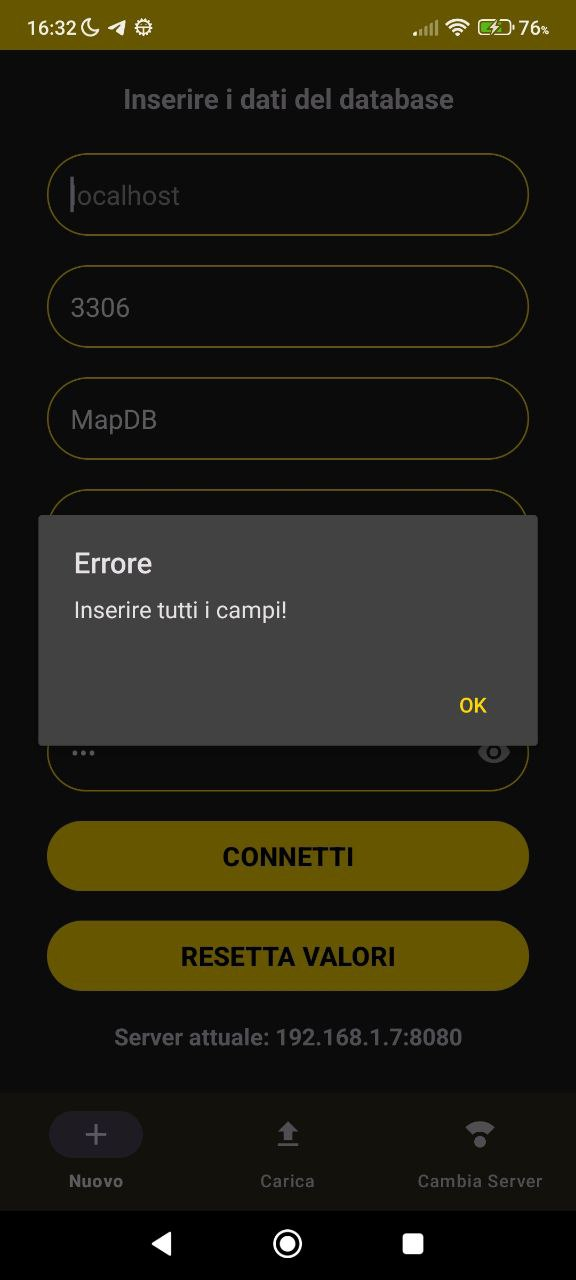
\includegraphics[scale=0.2]{img/app5.png}
    \end{figure}
    Se l'utente non compila correttamente qualche campo, riceverà un errore a seconda del campo non compilato correttamente.
    \begin{figure}[H]
      \centering
      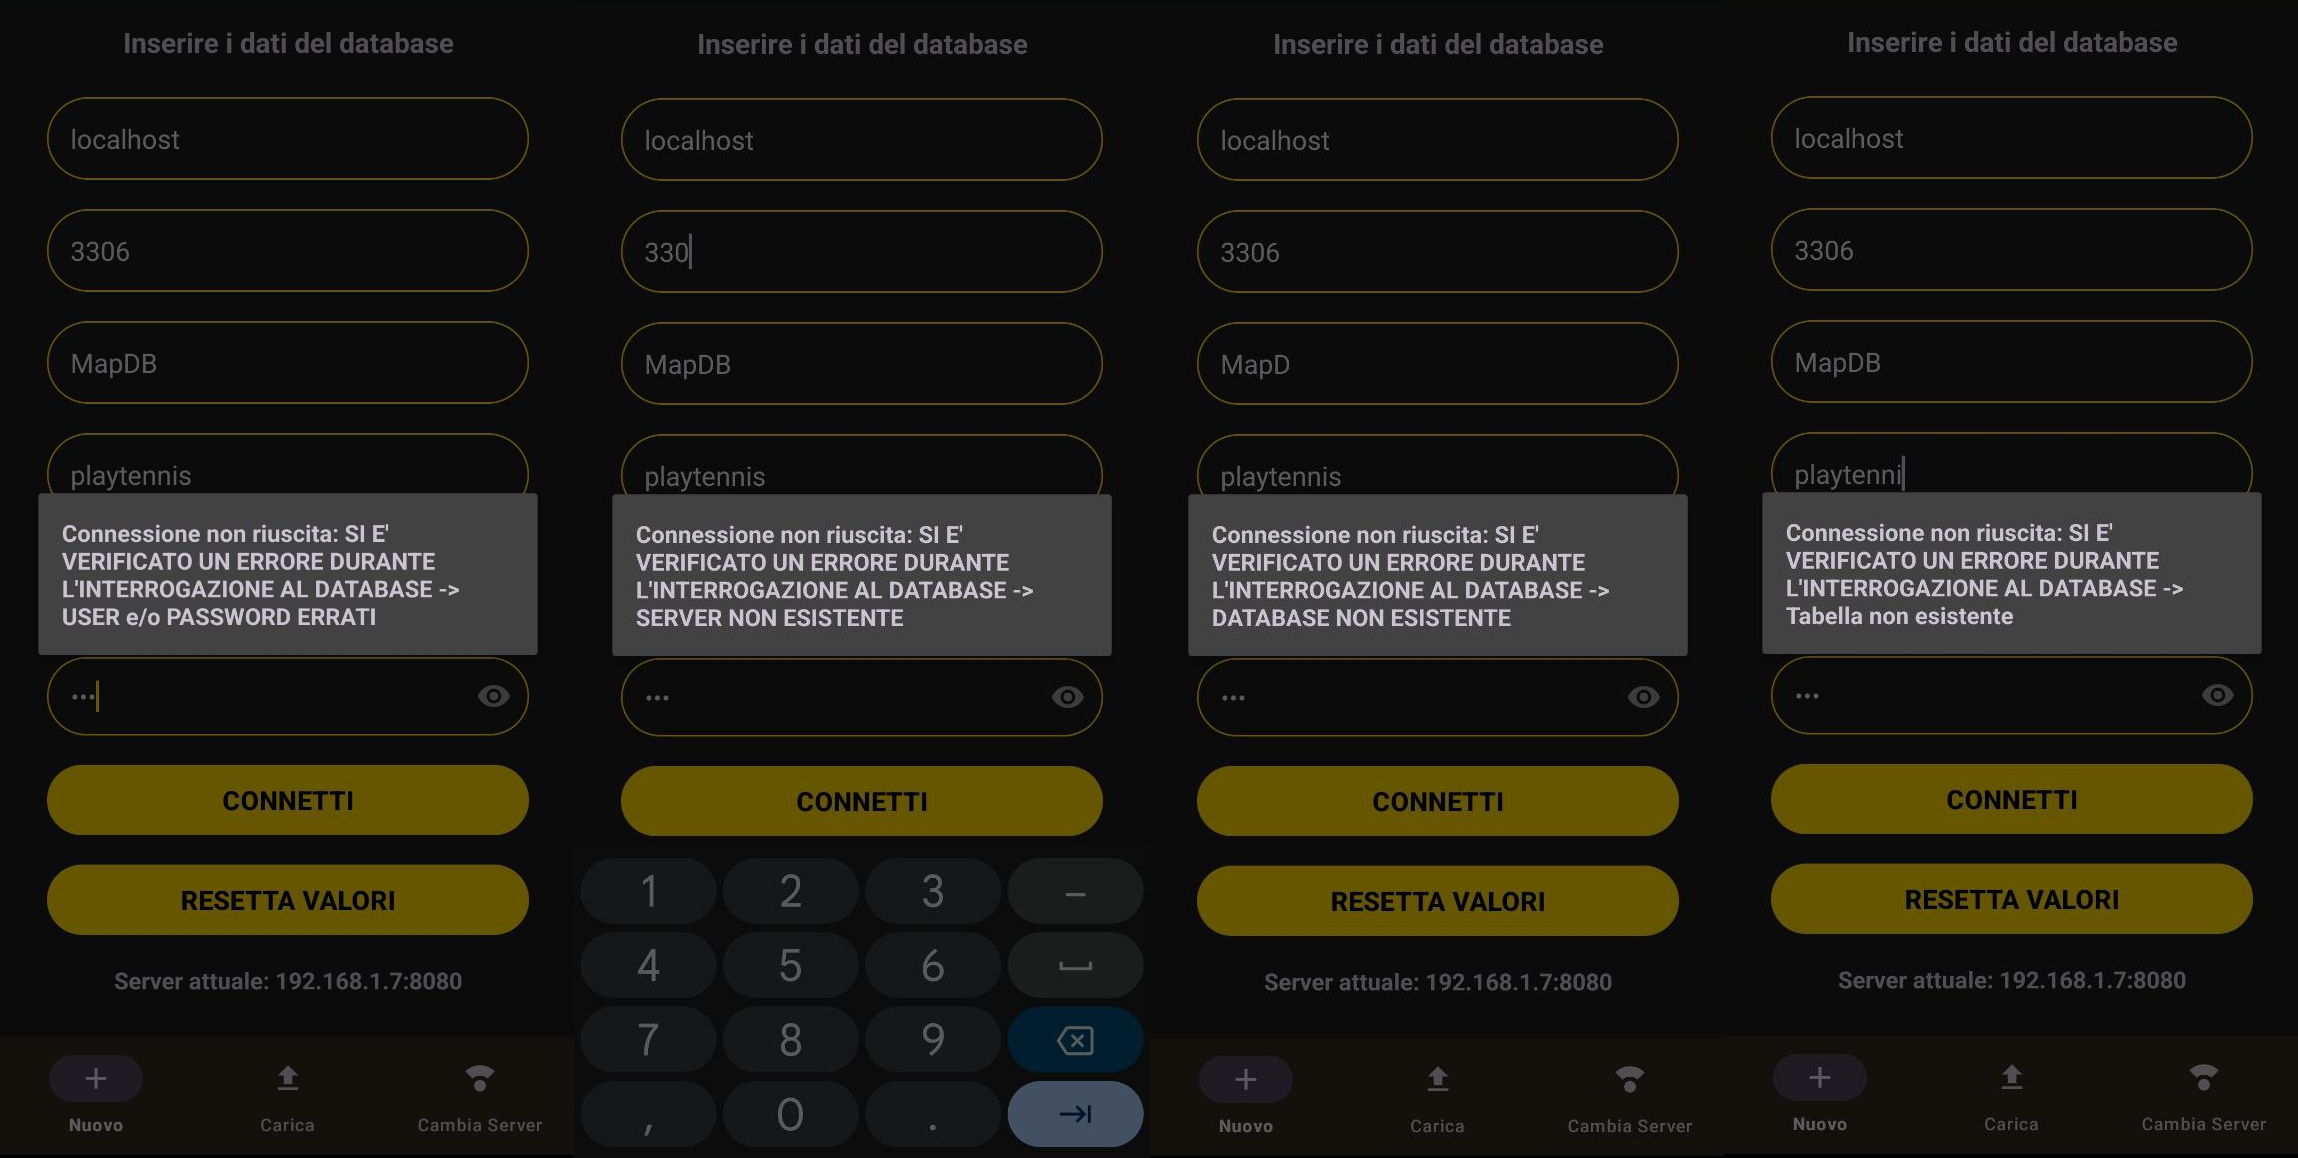
\includegraphics[scale=0.27]{img/app6.png}
    \end{figure}
  \end{itemize}
  \item \textbf{Esecuzione dell'algoritmo}: una volta selezionato il numero di cluster, l'applicazione eseguirà l'algoritmo di K-means quando viene premuto il pulsante e mostrerà all'utente i risultati. 
  \begin{figure}[H]
    \centering
    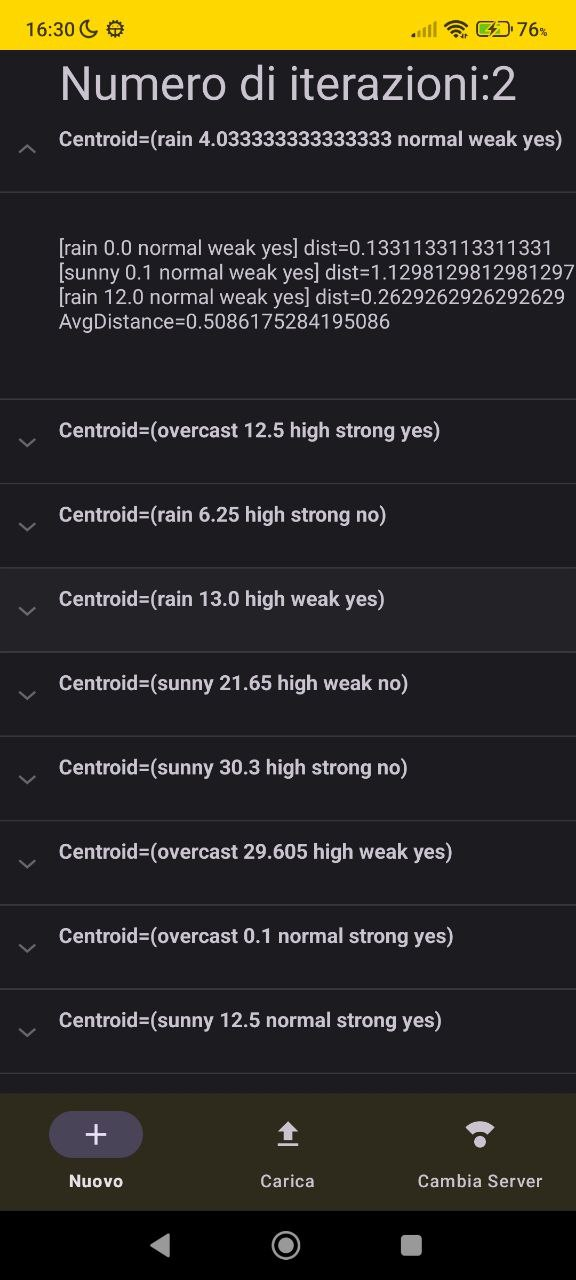
\includegraphics[scale=0.2]{img/app7.png}
  \end{figure}
  \item \textbf{Caricamento di un file}: l'utente può caricare un file di cluster serializzato sul server. Per farlo basta utilizzare l'apposito tab e cliccando su "Seleziona un file" l'utente può scegliere il file da caricare dall'elenco dei file presenti sul server. 
  \begin{figure}[H]
    \centering
    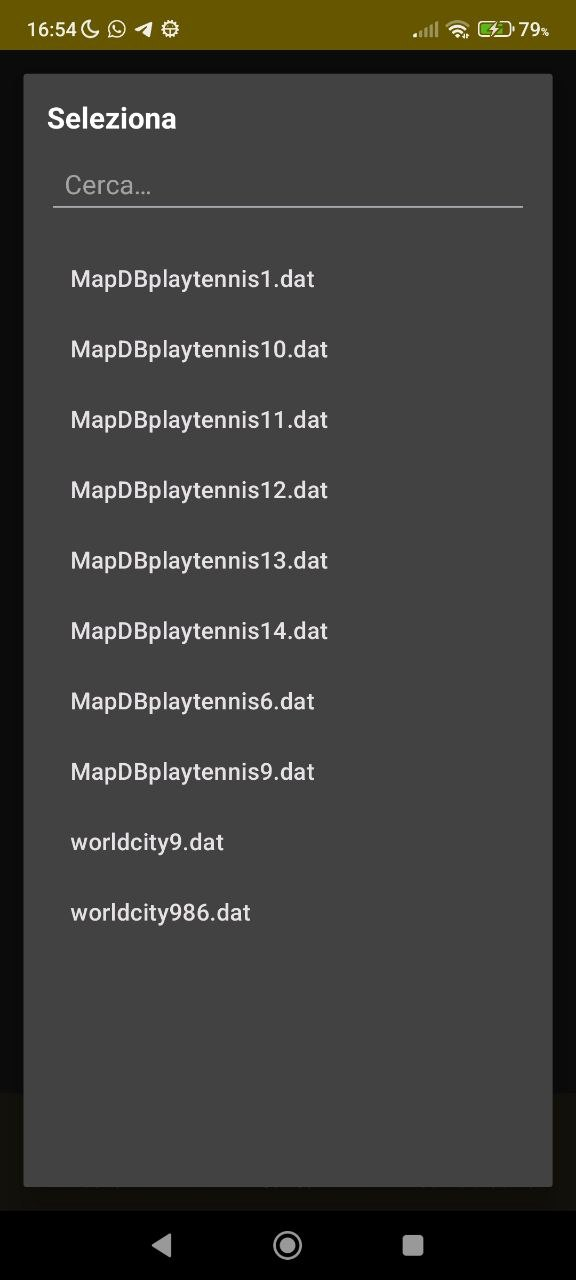
\includegraphics[scale=0.2]{img/app8.png}
  \end{figure}
  Nel caso in cui vi sia un file non valido lato server, o se l'utente non sceglie alcun file, cliccando il pulsante "Recupera file" riceverà un errore. 
  \begin{figure}[H]
    \centering
    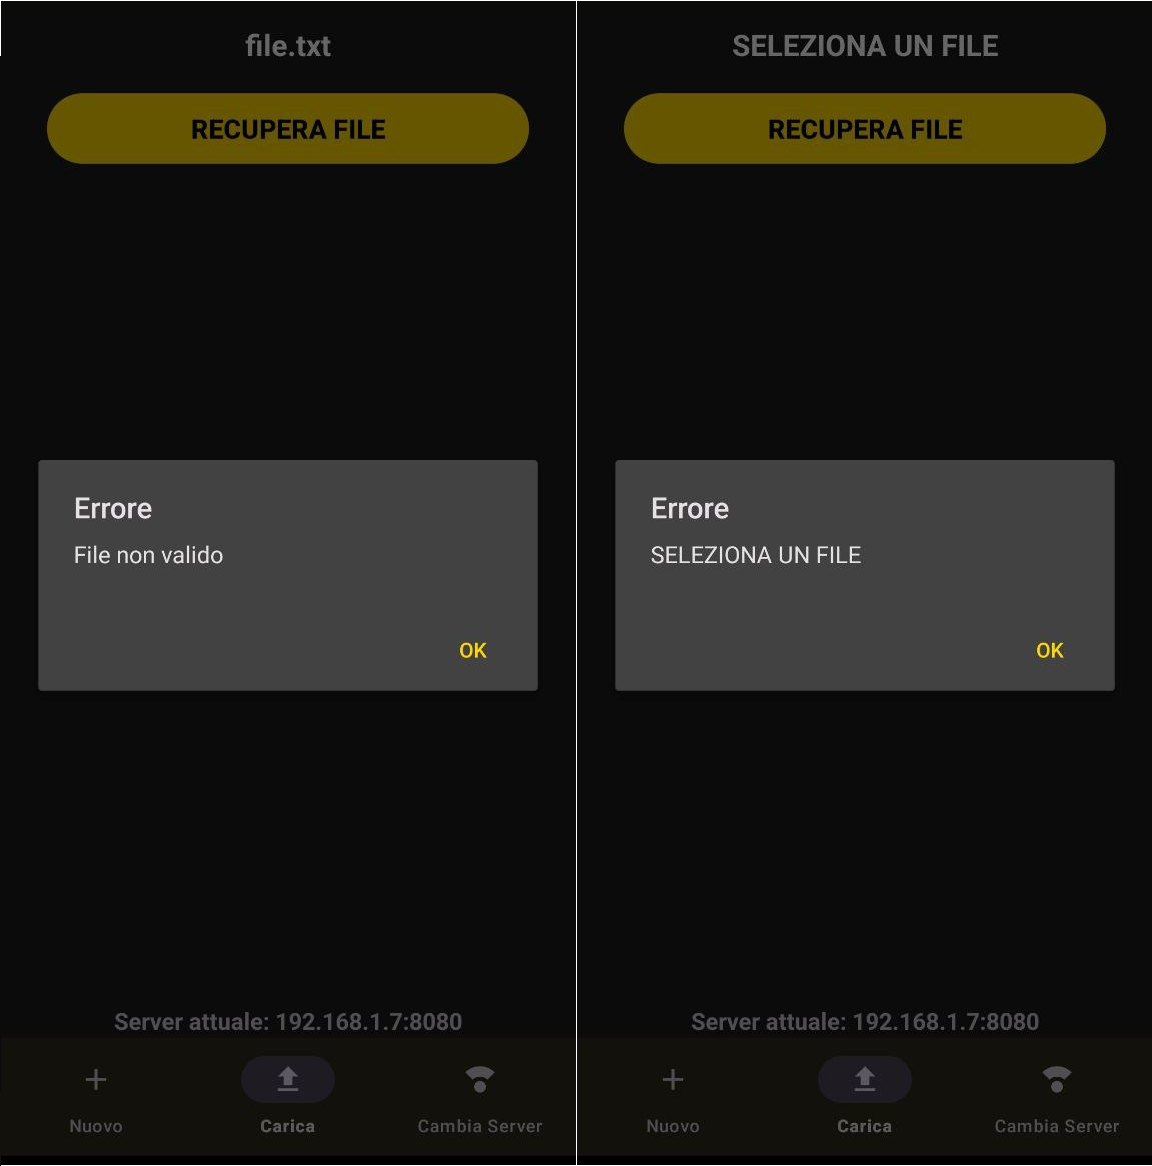
\includegraphics[scale=0.35]{img/app9.png}
  \end{figure}
  Se il server non è corretto, l'utente riceverà un errore nel momento in cui proverà ad aprire l'elenco dei file.
  \begin{figure}[H]
    \centering
    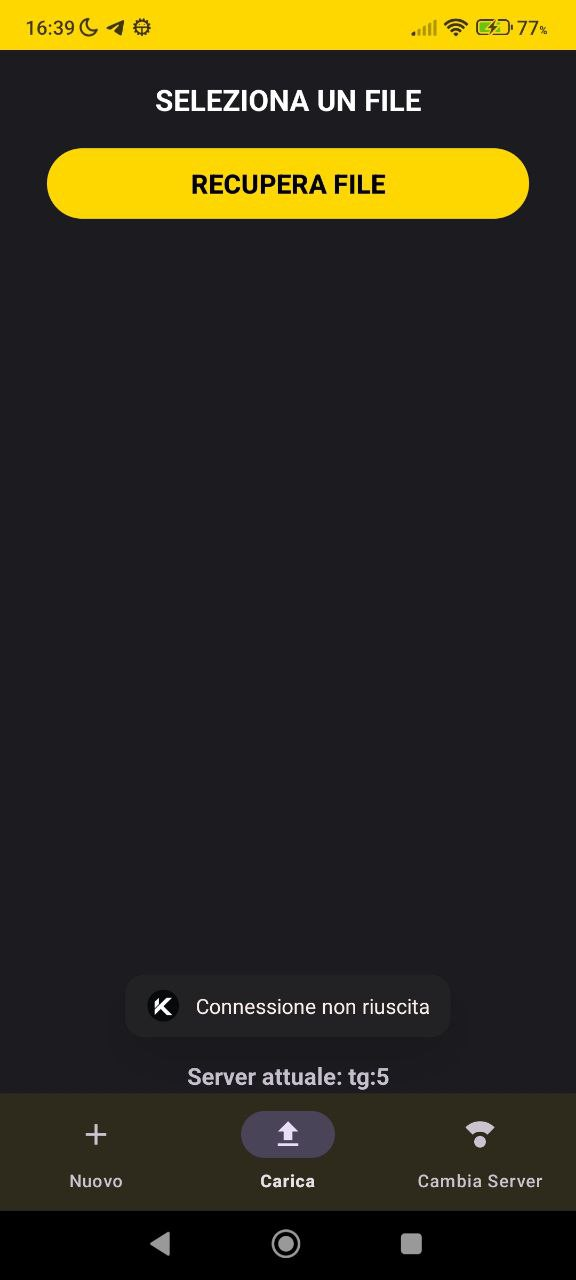
\includegraphics[scale=0.2]{img/app10.png}
  \end{figure}
  \item \textbf{Cambio server}: nell'apposito tab l'utente può cambiare il server a cui connettersi. Nel caso in cui non vengano compilati tutti i campi, l'utente riceverà un errore.
  \begin{figure}[H]
    \centering
    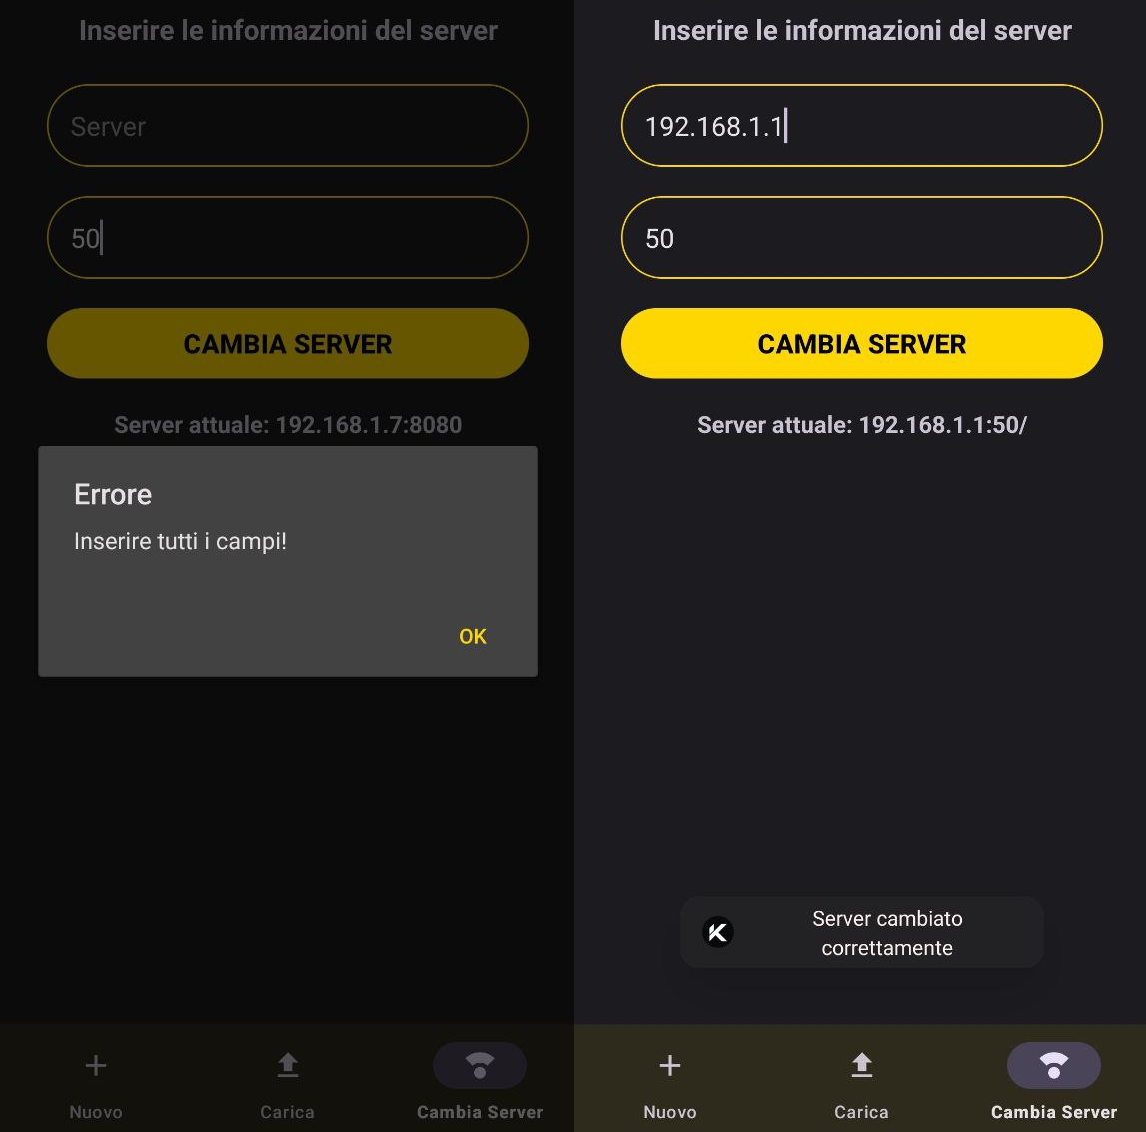
\includegraphics[scale=0.35]{img/app11.png}
  \end{figure}
  \item \textbf{Passaggio di un numero di cluster non valido}: non è possibile dal client app passare un numero di cluster non valido, ma nell'eventualità in cui ciò accada, il server è in grado di gestire l'eccezione inviando un errore.
  \begin{figure}[H]
    \centering
    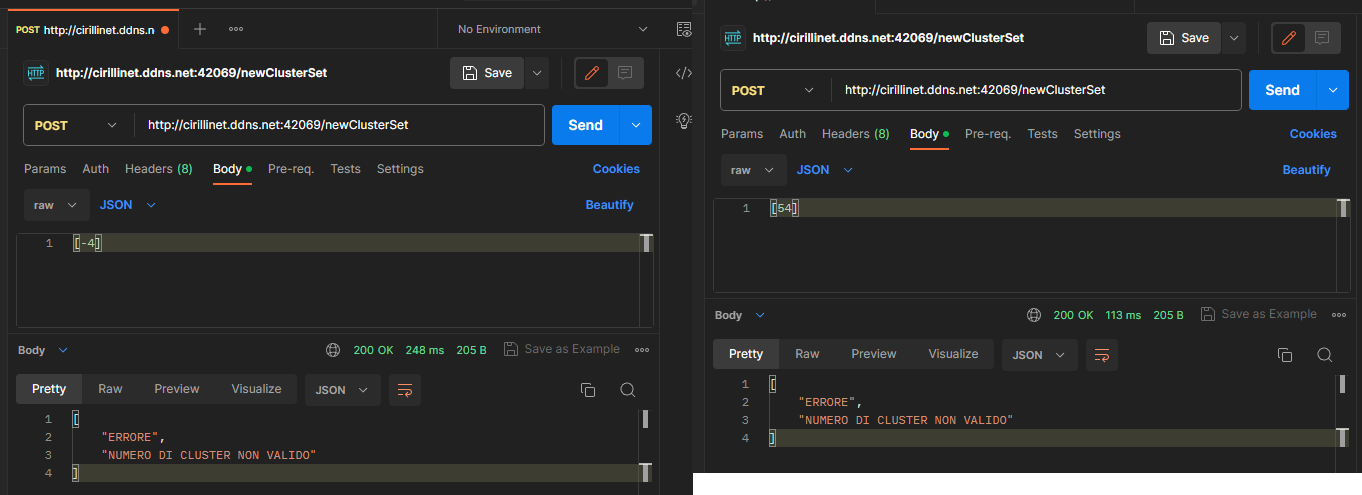
\includegraphics[scale=0.4]{img/app12.png}
  \end{figure}
\end{enumerate}